\subsection{شبیه‌سازی کانال رول استند در حضور کنترل‌کننده LQIDG}\label{roll_lqidg_section}
در بخش
\ref{quadchanell_roll}
شبیه‌سازی کانال رول استند چهارپره انجام شد. در این بخش به بررسی عملکرد چهارپره در حضور کنترل‌کننده LQIDG پرداخته می‌شود. کنترل‌کننده LQDG در بخش‌های
\ref{openloop_game}
و
\ref{closedloop_game}
بررسی شده است.
 در شبیه‌سازی برای بهینه‌سازی ضرایب وزنی از روش
TCACS \cite{Karimi2010}
استفاده شده است.
\

\begin{figure}[H]
	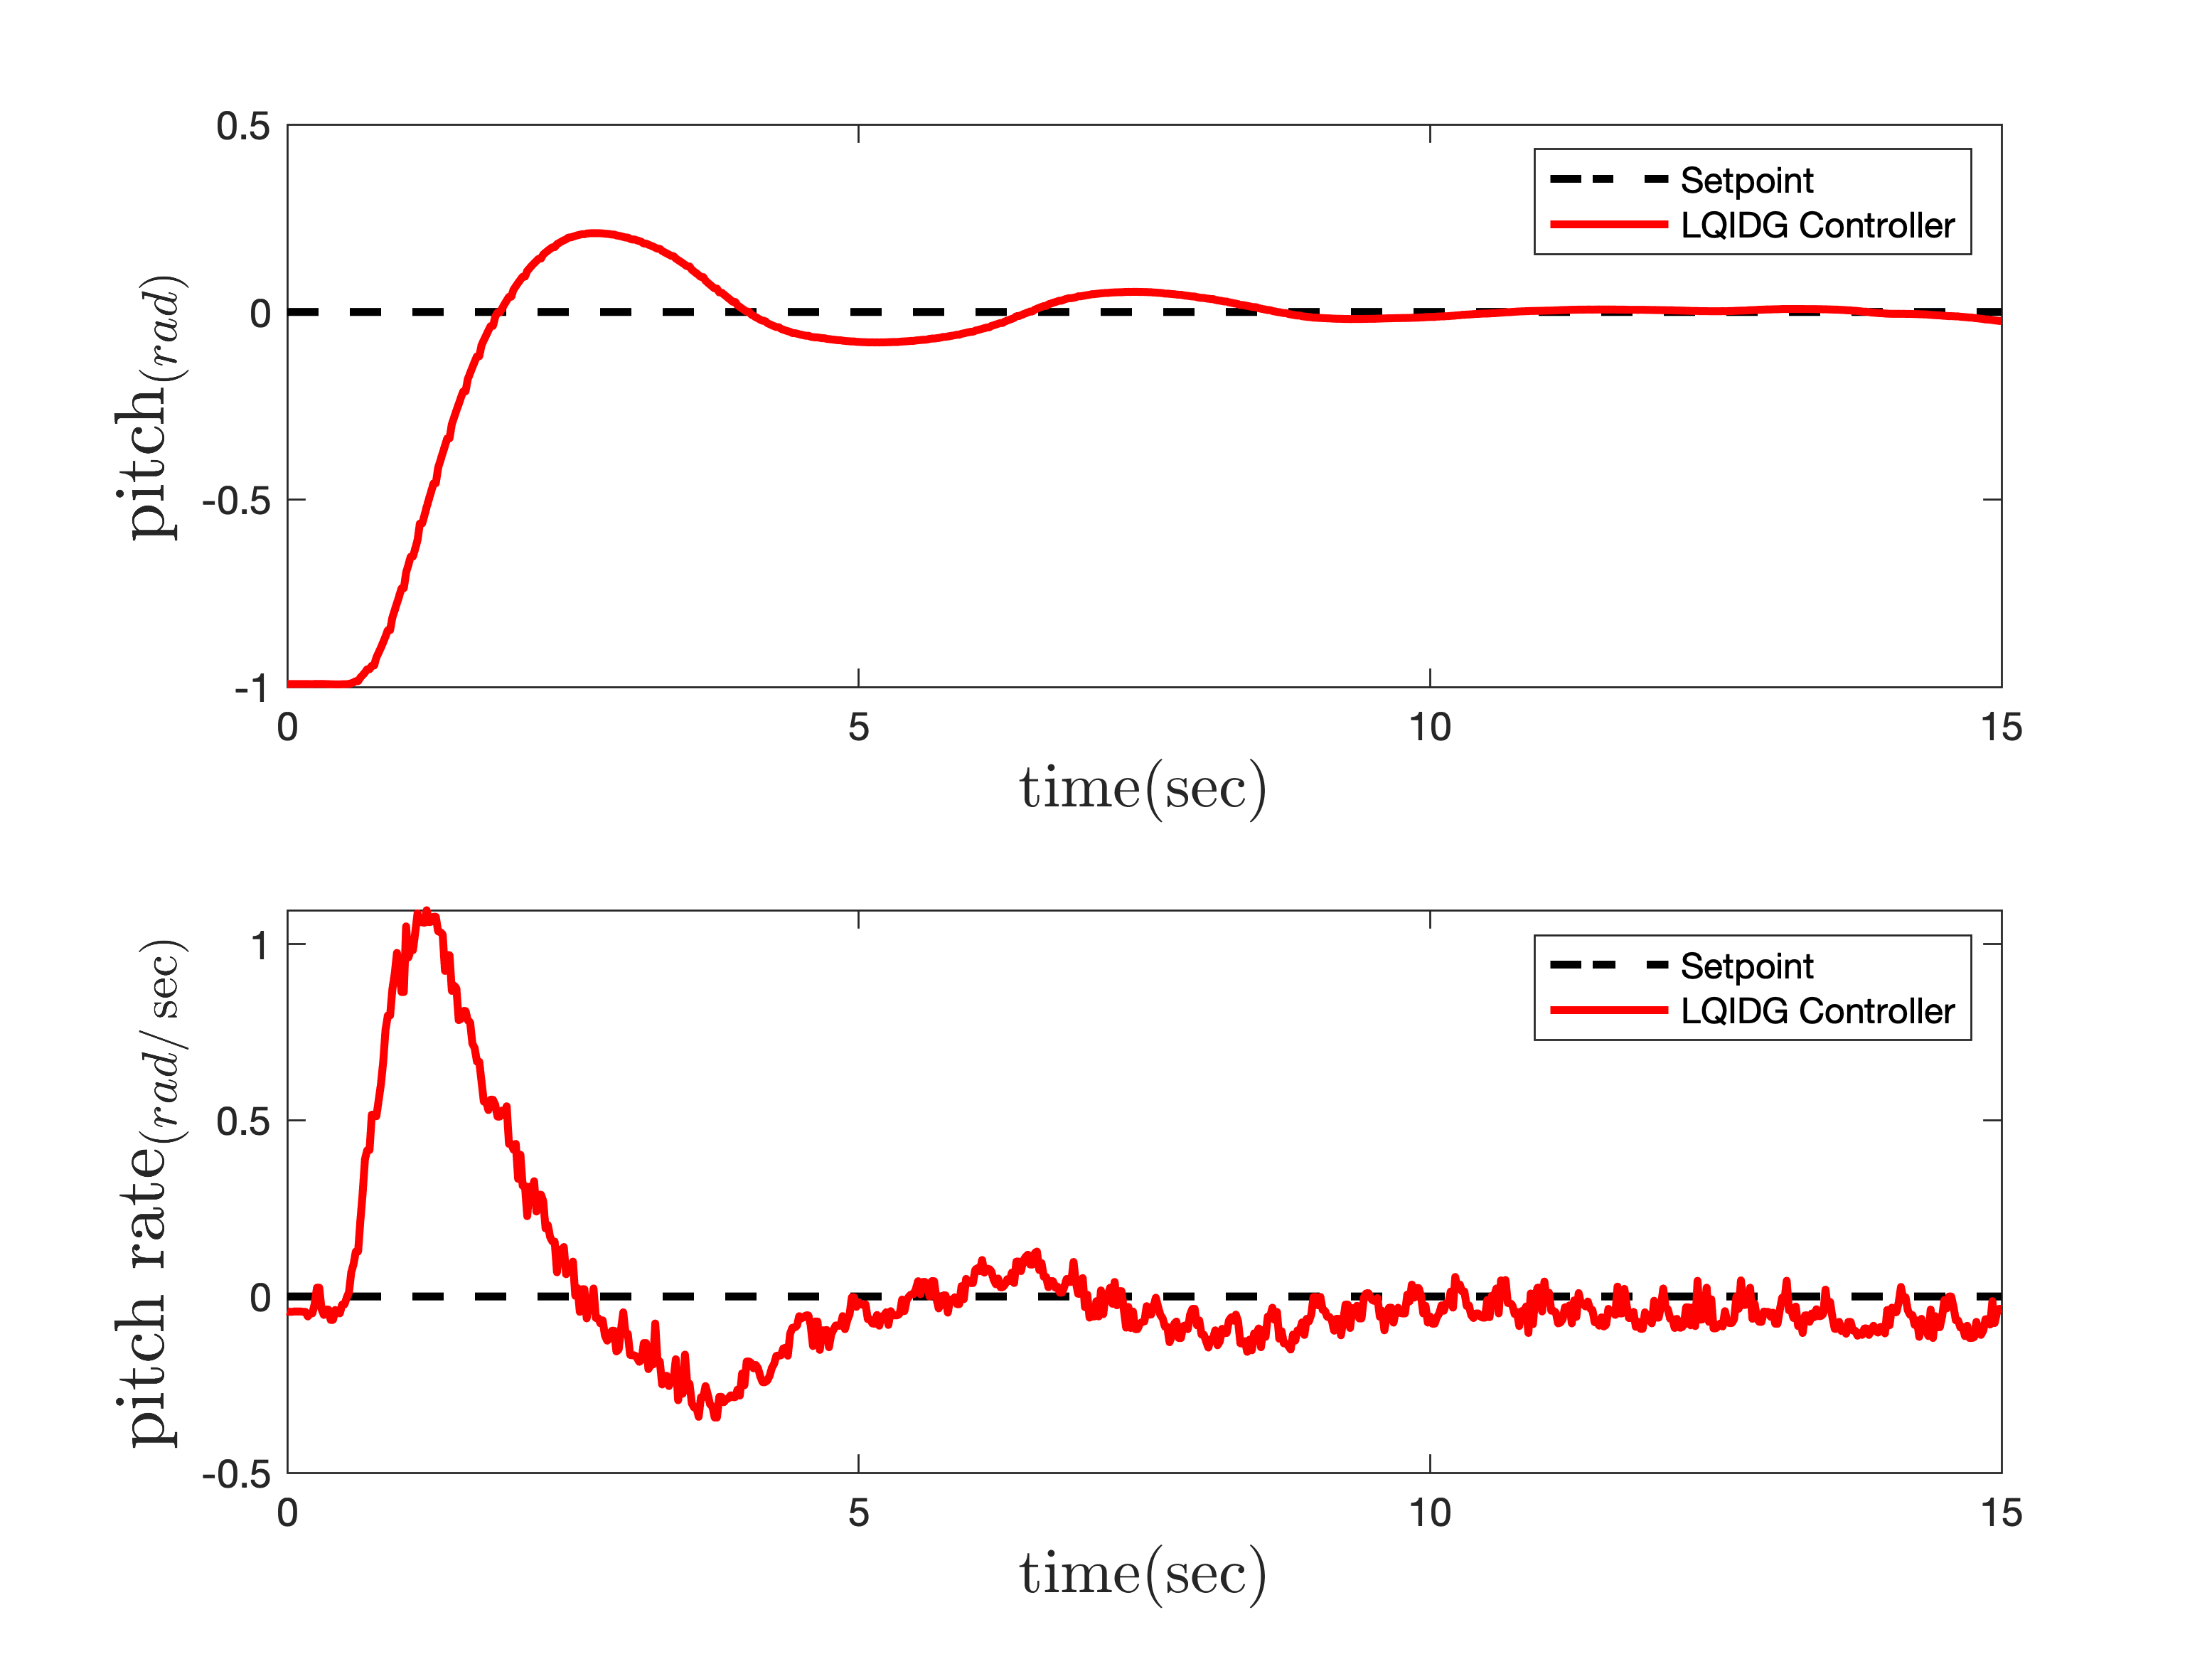
\includegraphics[width=.6\linewidth]{../Figures/Calibration/LQIDG/Pitch/lqidg_pitch.png}
	\centering
	\caption{عملكرد LQIDG در کنترل زاويه رول (تعقیب ورودی صفر)}
\end{figure}

%\begin{figure}
%	[width=12cm]
%	\centering
%	\begin{subfigure}
%		\centering
%		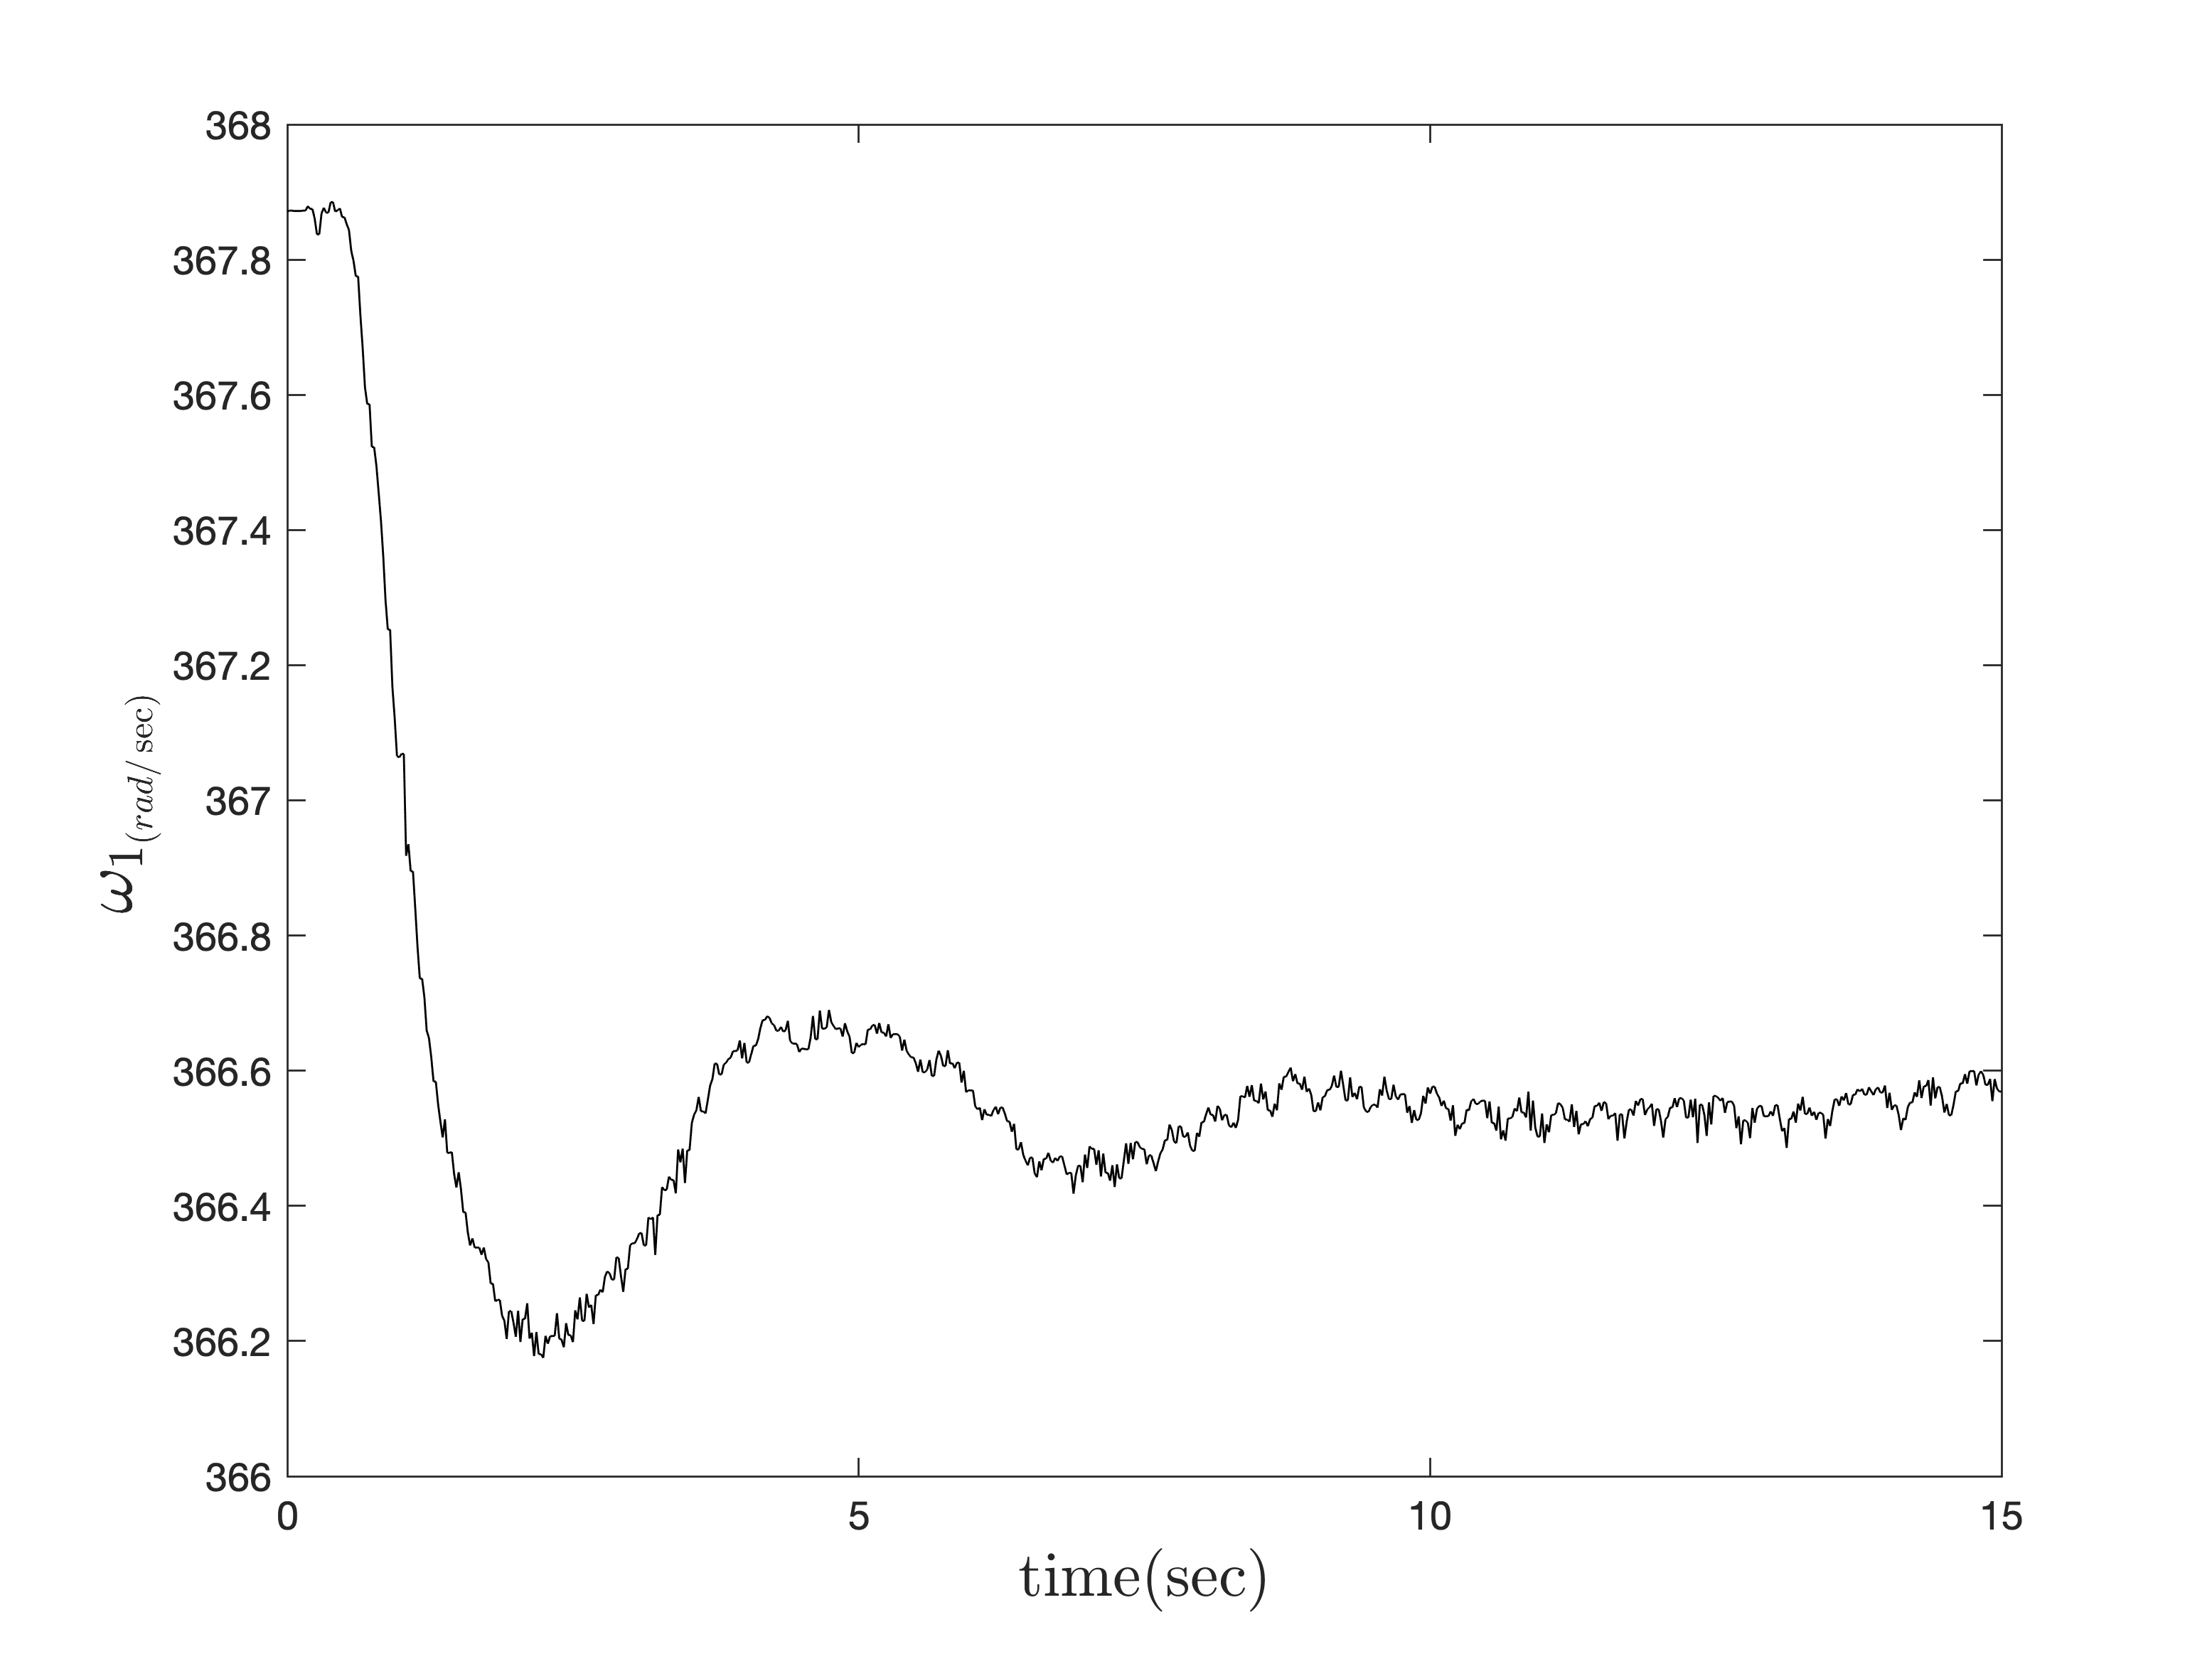
\includegraphics[width=12cm]{../Figures/Calibration/LQIDG/Pitch/lqidg_Omega_1.png}
%		\caption{موتور شماره یک}
%	\end{subfigure}
%	\begin{subfigure}
%		\centering
%		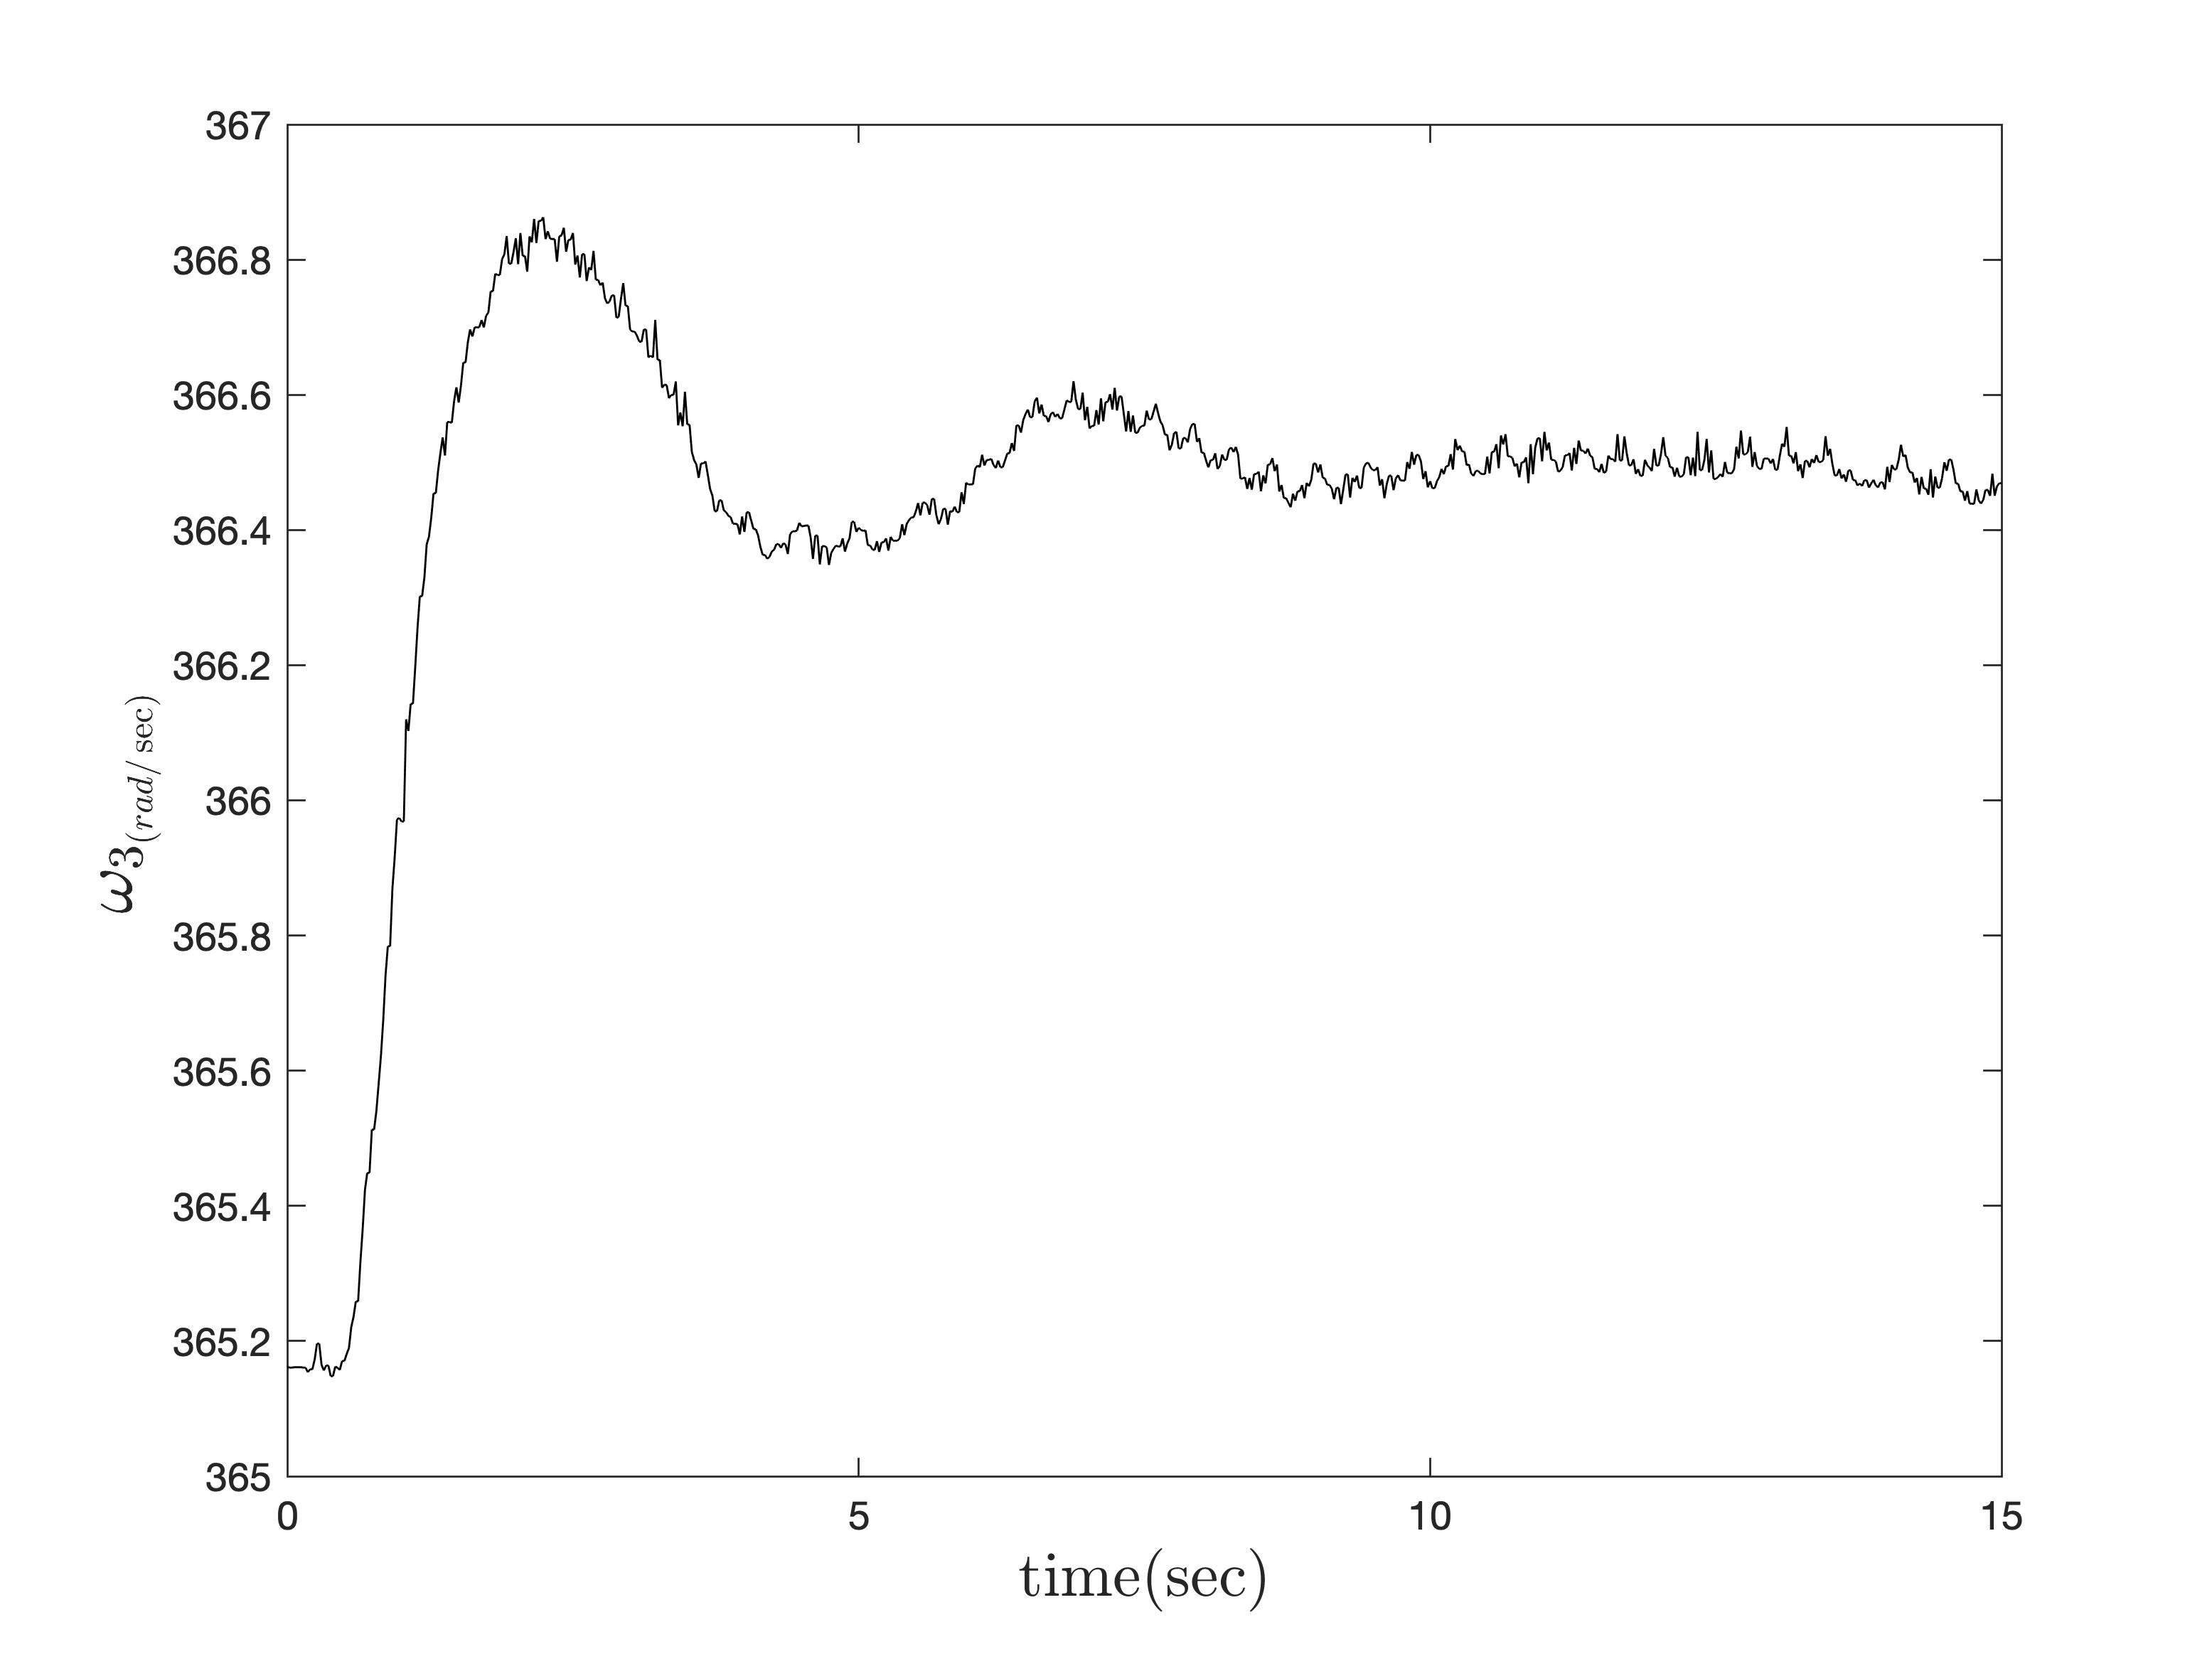
\includegraphics[width=12cm]{../Figures/Calibration/LQIDG/Pitch/lqidg_Omega_3.png}
%		\caption{موتور شماره سه}
%	\end{subfigure}
%	\caption{‫‪فرمان کنترل‌کننده موتور سه و چهار در کنترل زاویه رول و پیچ (تعقیب ورودی صفر)}
%\end{figure}

\begin{figure}[H]
	\centering
	\subfigure[موتور شماره یک]{
		\centering
		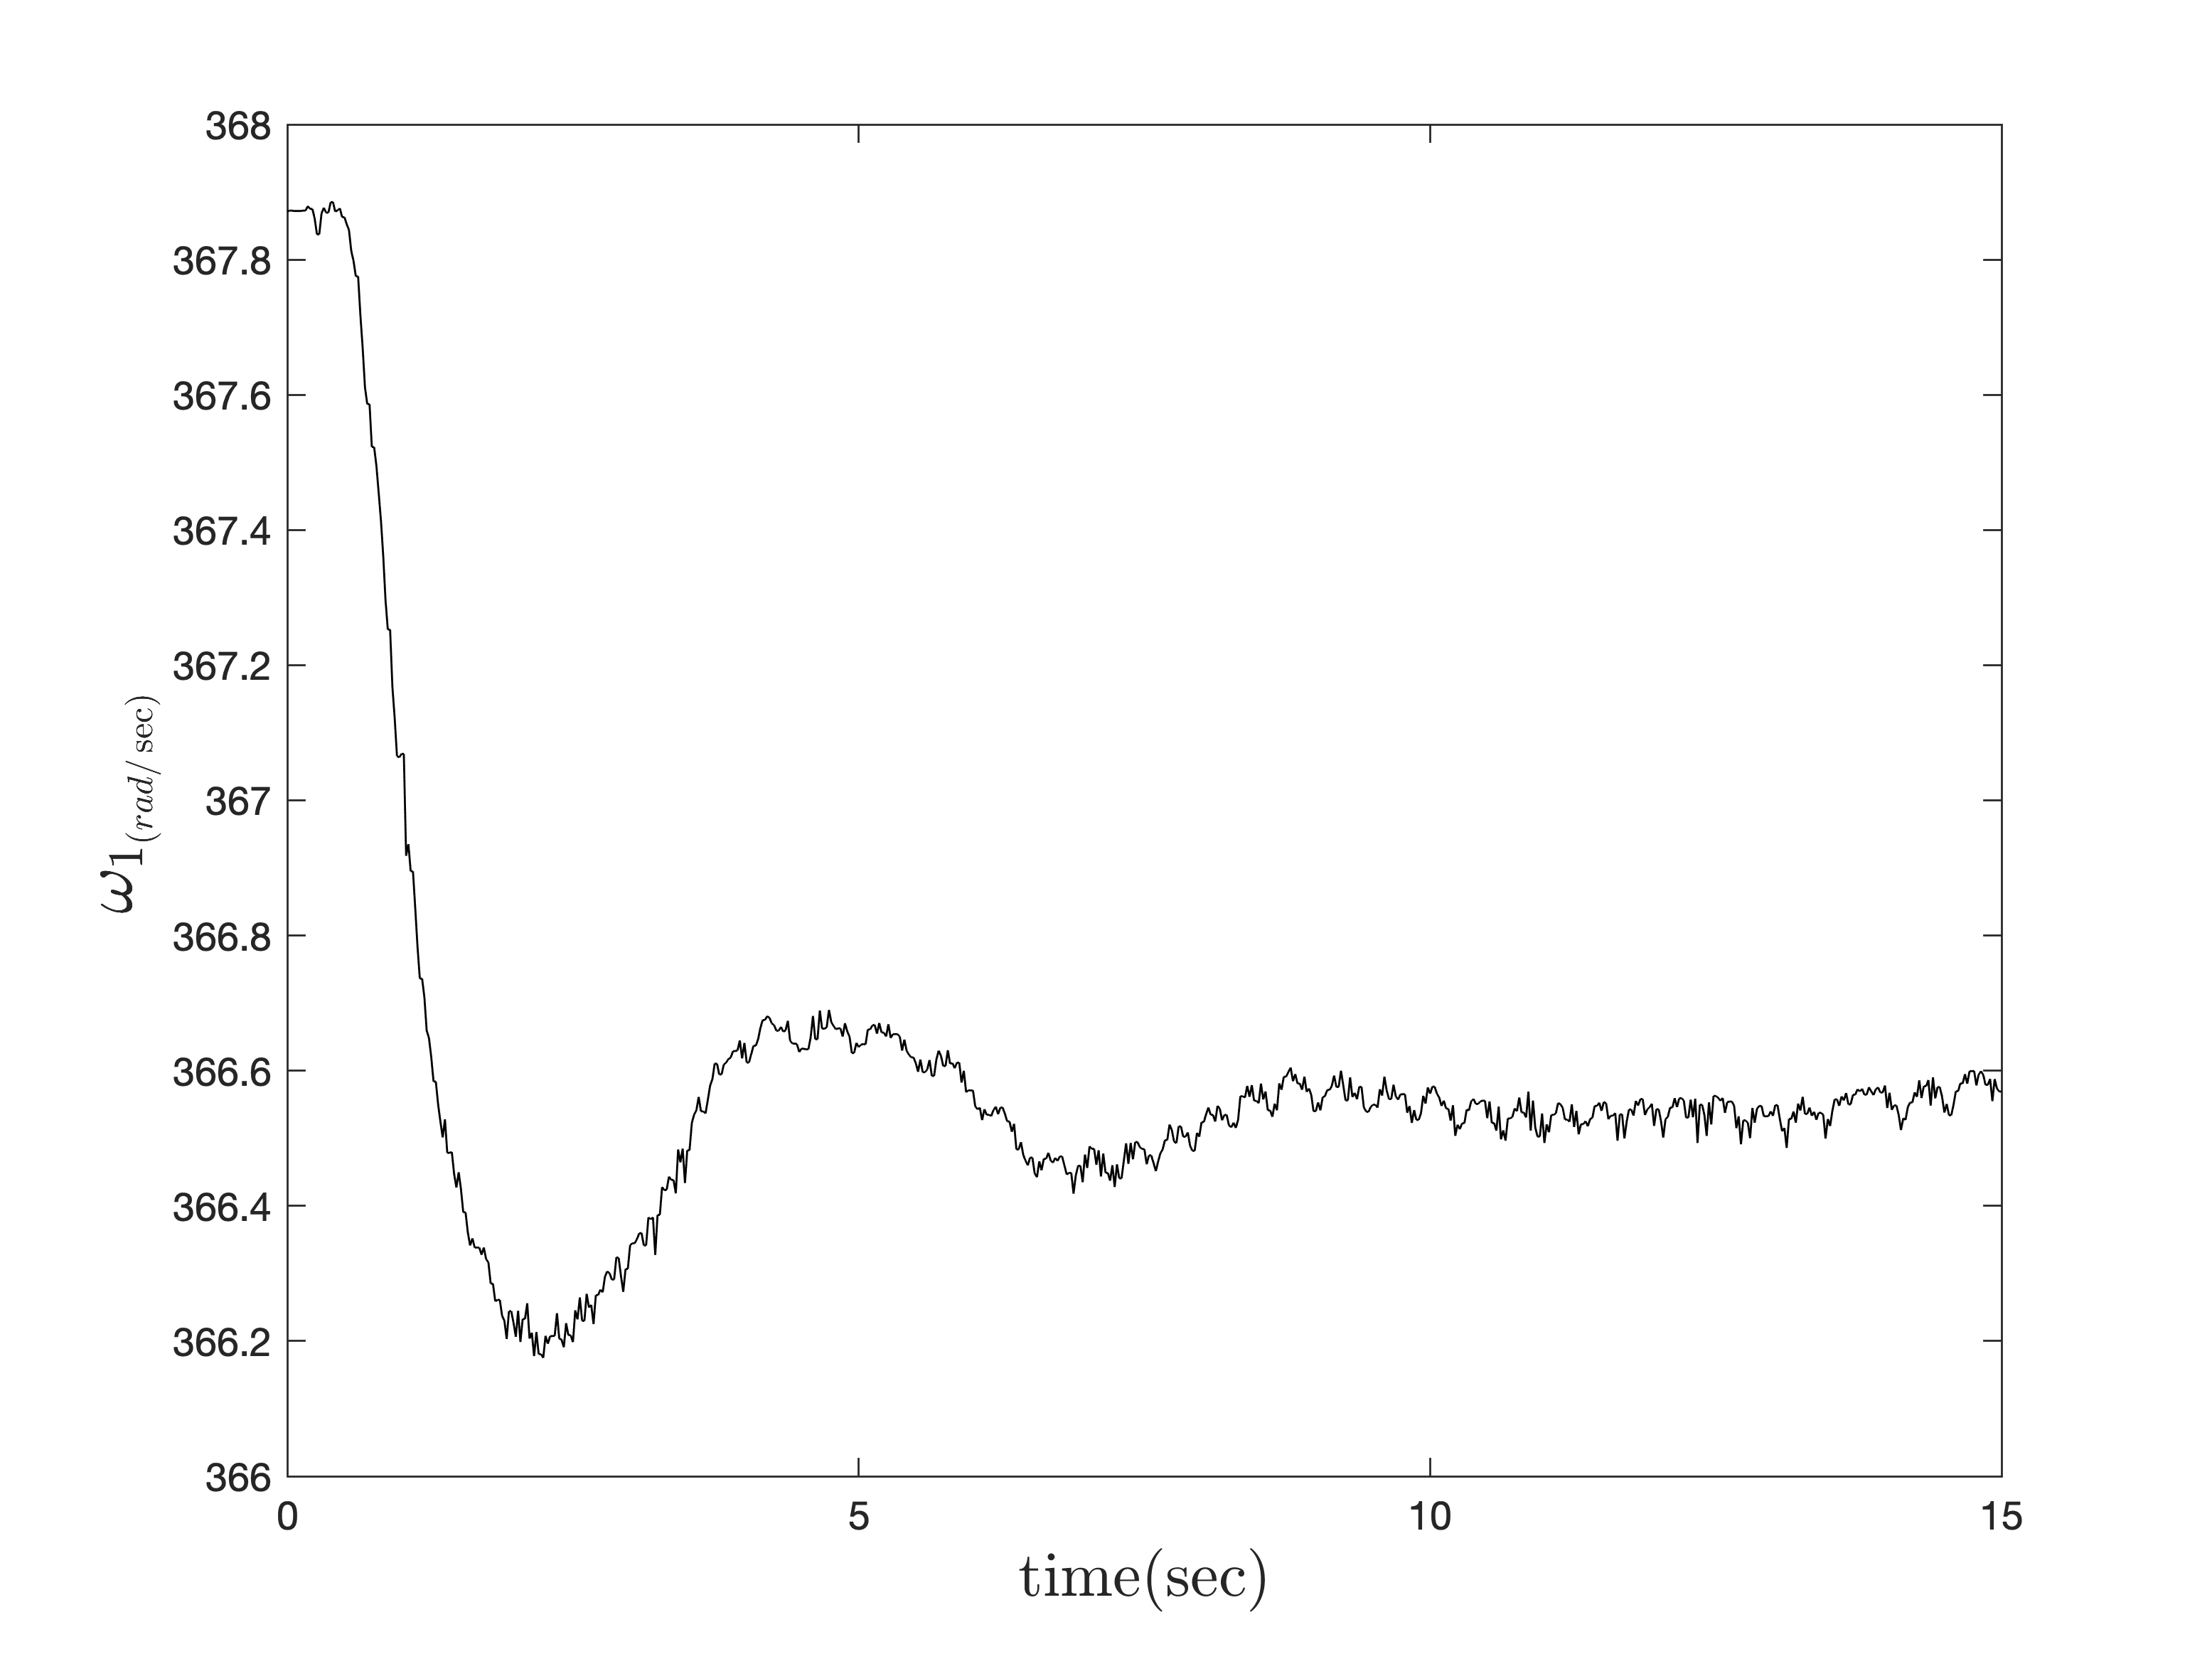
\includegraphics[width=.45\linewidth]{../Figures/Calibration/LQIDG/Pitch/lqidg_Omega_1.png}
	}
	\subfigure[موتور شماره سه]{
		\centering
		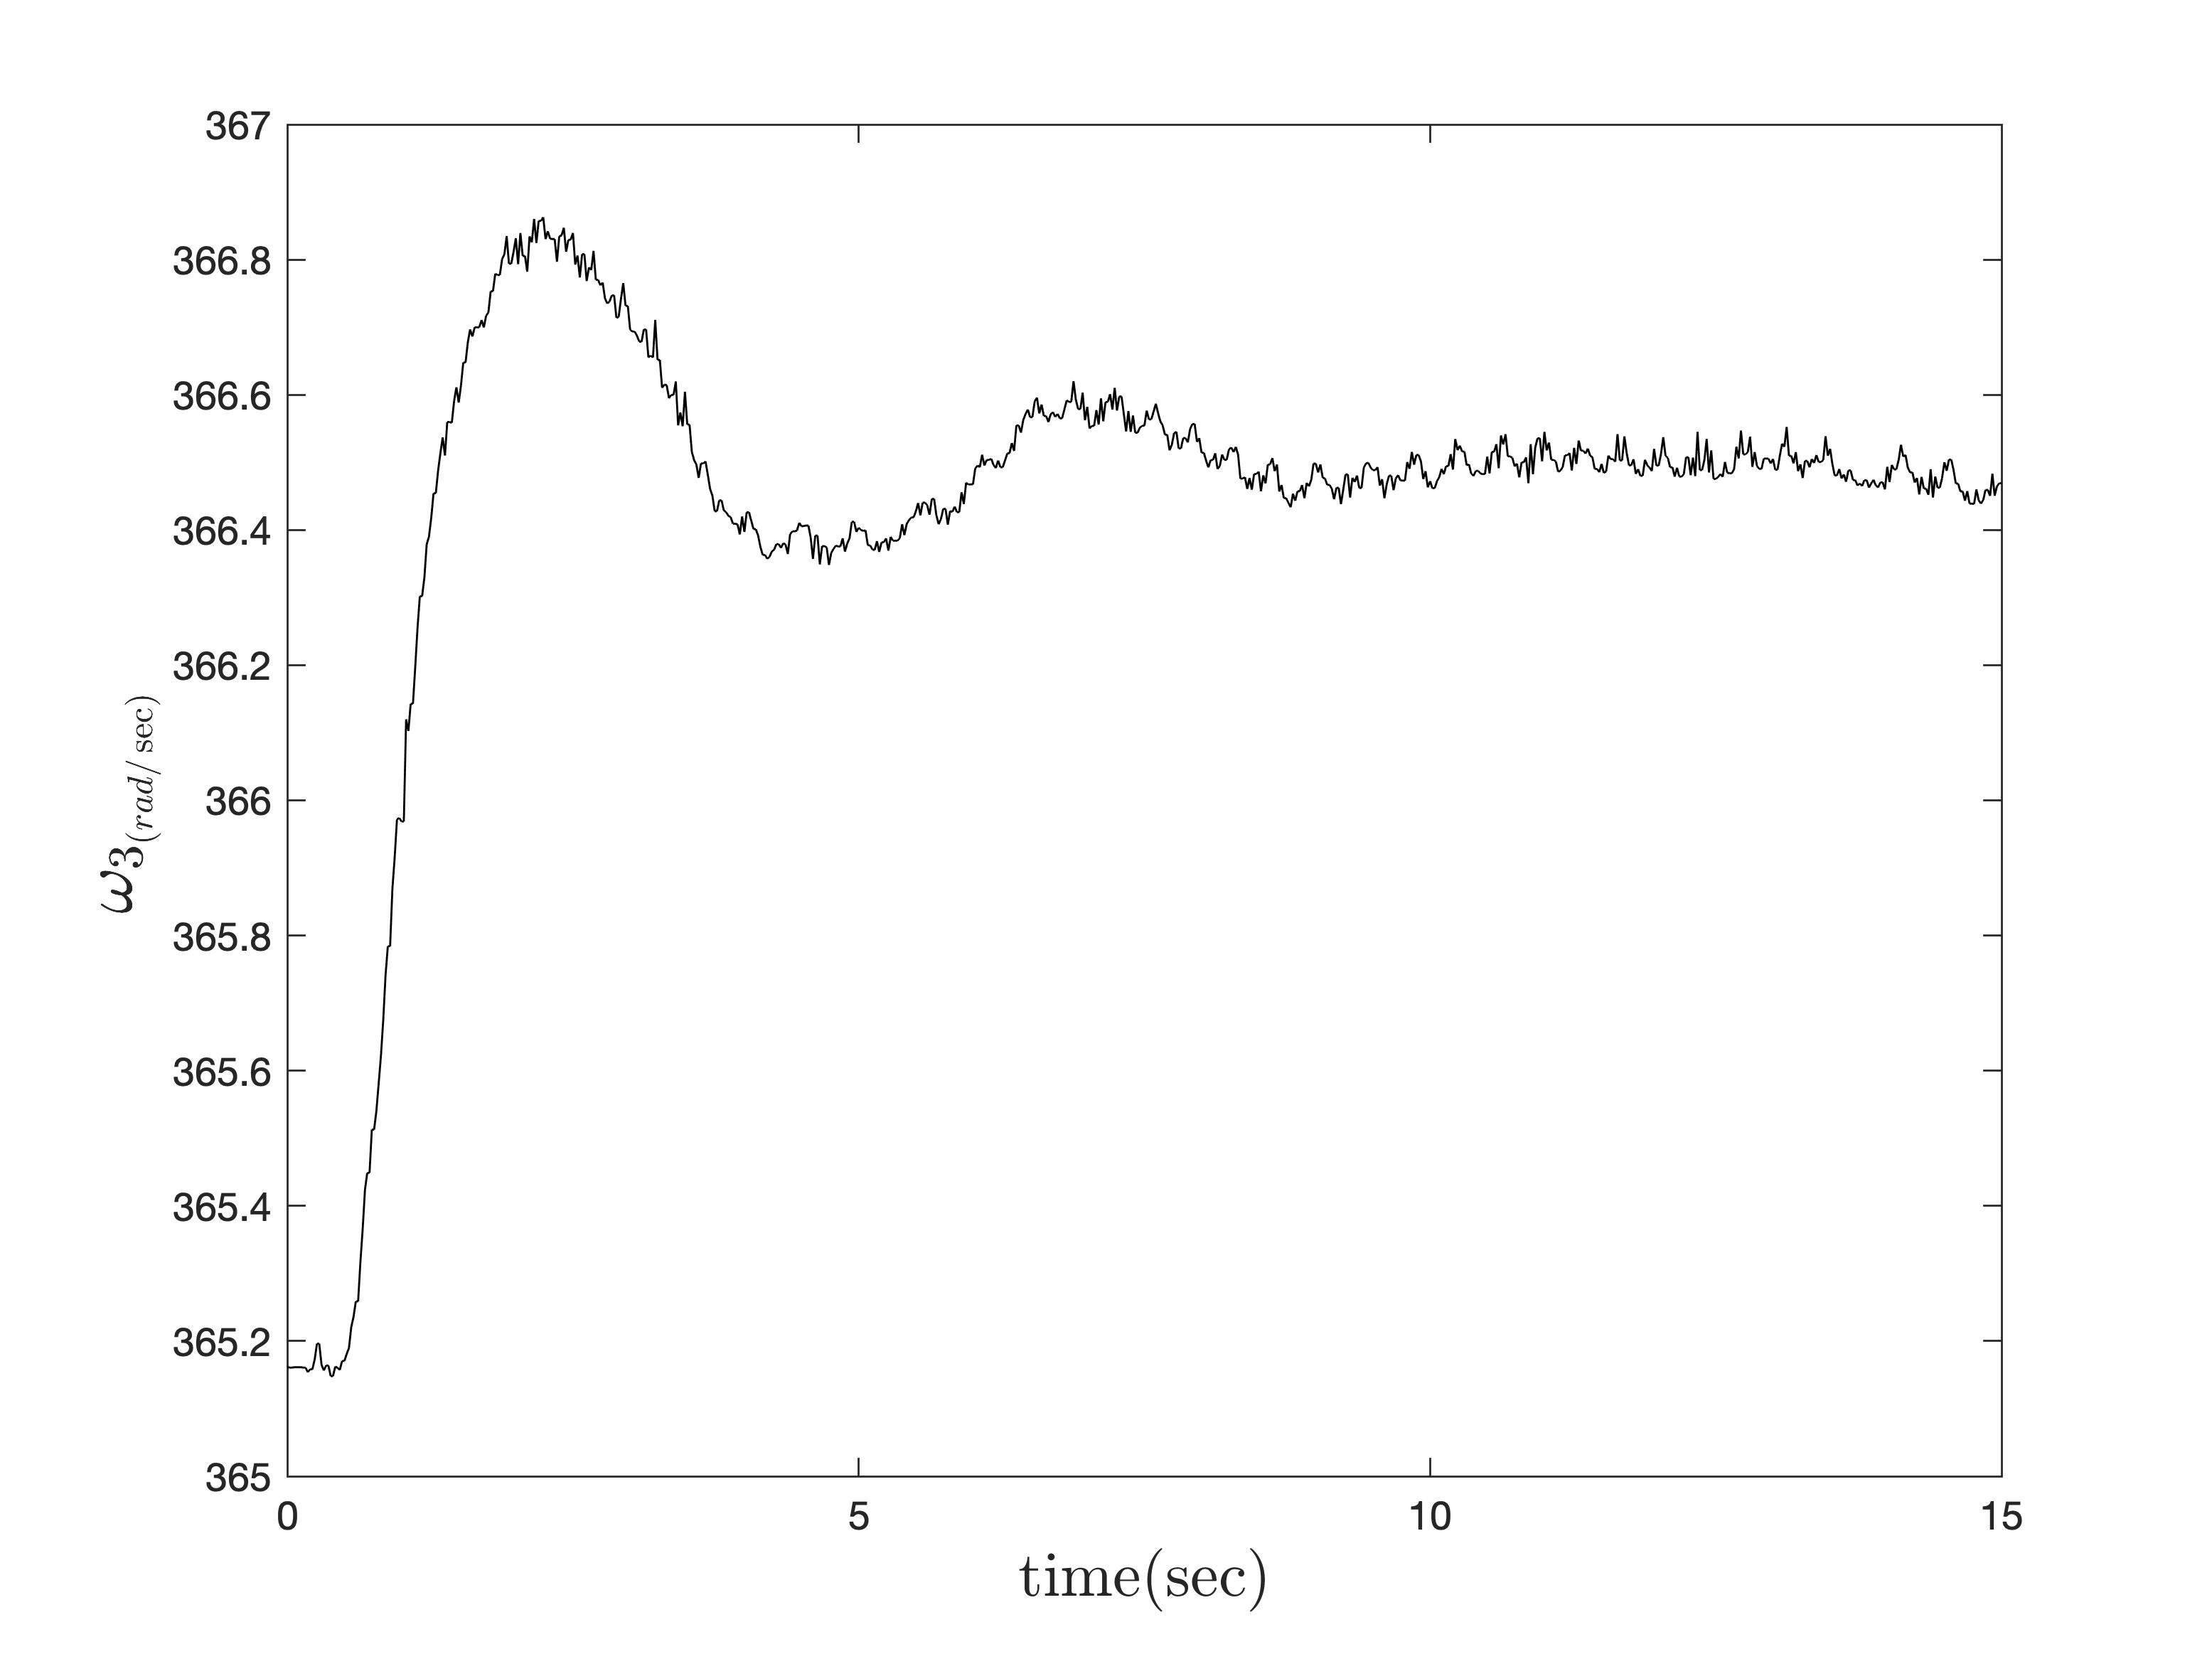
\includegraphics[width=.45\linewidth]{../Figures/Calibration/LQIDG/Pitch/lqidg_Omega_3.png}
	}
	\caption{‫‪فرمان کنترلی موتورها در کنترل زاویه پیچ (تعقیب ورودی صفر)}
\end{figure}



بر اساس خروجی شبیه‌سازی (شکل
\ref{lqidg_roll_fig})
،کانال رول در حضور کنترل‌کننده LQIDG در حدود پنج ثانیه به تعادل می‌رسد و خطای ماندگار آن در حدود صفر است.